\documentclass[tikz,border=4pt]{standalone}
\usepackage[T1]{fontenc}
\usepackage[utf8]{inputenc}
\usepackage{tikz}
\usetikzlibrary{arrows.meta,positioning}

\definecolor{calyrbg}{RGB}{14,18,24}
\definecolor{calyrpanel}{RGB}{24,30,39}
\definecolor{calyrink}{RGB}{235,239,244}
\definecolor{calyrmuted}{RGB}{150,161,173}
\definecolor{calyraccent}{RGB}{92,203,255}
\definecolor{calyrline}{RGB}{45,57,72}
\definecolor{MagentaAI}{RGB}{214,116,255}

\begin{document}
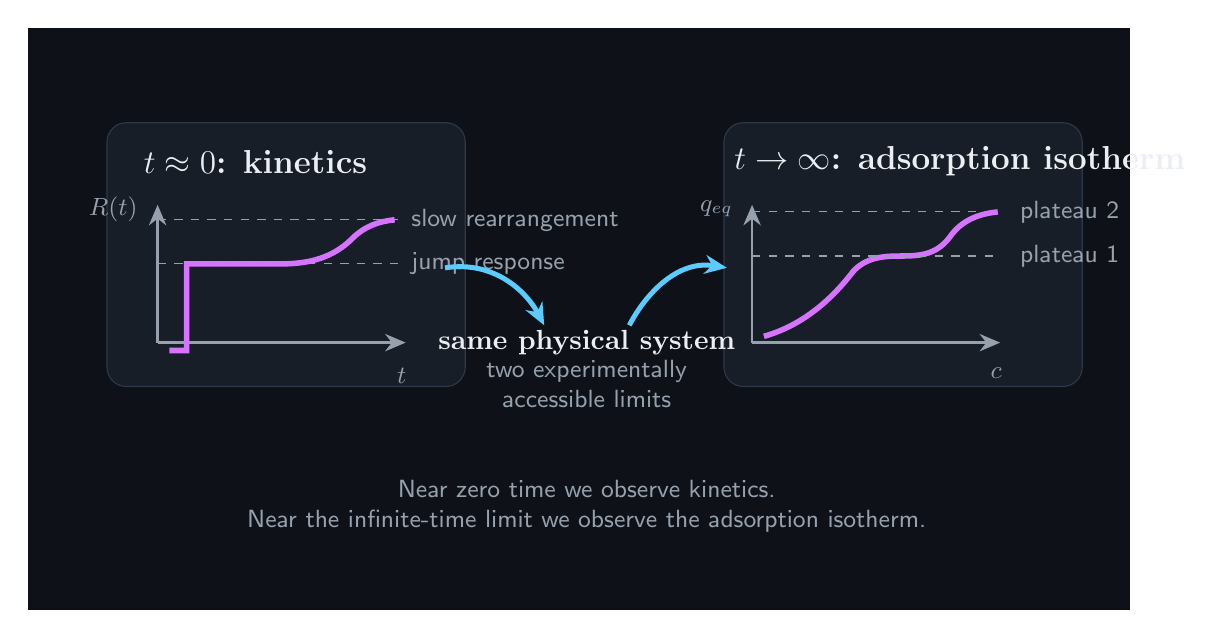
\begin{tikzpicture}[
  font=\sffamily\small,
  axis/.style={draw=calyrmuted, line width=0.9pt, -{Stealth[length=2.6mm,width=2.2mm]}},
  curve/.style={draw=MagentaAI, line width=2pt},
  bridge/.style={draw=calyraccent, line width=1.8pt, -{Stealth[length=2.8mm,width=2.4mm]}},
  panel/.style={draw=calyrline, fill=calyrpanel, rounded corners=7pt}
]
\fill[calyrbg] (-0.4,-0.4) rectangle (13.6,7.0);

\node[panel, minimum width=4.55cm, minimum height=3.35cm, anchor=north west] (leftpanel) at (0.6,5.8) {};
\node[panel, minimum width=4.55cm, minimum height=3.35cm, anchor=north east] (rightpanel) at (13.0,5.8) {};

\node[anchor=west, text=calyrink, font=\bfseries\large] at (0.95,5.3) {$t \approx 0$: kinetics};
\node[anchor=west, text=calyrink, font=\bfseries\large] at (8.45,5.3) {$t \to \infty$: adsorption isotherm};

\draw[axis] (1.25,3.0) -- (1.25,4.75);
\draw[axis] (1.25,3.0) -- (4.4,3.0);
\node[text=calyrmuted, anchor=east] at (1.12,4.7) {$R(t)$};
\node[text=calyrmuted, anchor=north] at (4.35,2.8) {$t$};
\draw[curve] (1.4,2.9) -- (1.62,2.9) -- (1.62,4.0)
             .. controls (1.98,4.0) and (2.45,4.0) .. (2.82,4.0)
             .. controls (3.18,4.0) and (3.48,4.08) .. (3.72,4.32)
             .. controls (3.88,4.48) and (4.06,4.54) .. (4.26,4.56);
\draw[dashed, color=calyrmuted] (1.25,4.0) -- (4.3,4.0);
\draw[dashed, color=calyrmuted] (1.25,4.56) -- (4.3,4.56);
\node[text=calyrmuted, anchor=west] at (4.35,4.0) {jump response};
\node[text=calyrmuted, anchor=west] at (4.35,4.56) {slow rearrangement};

\draw[axis] (8.8,3.0) -- (8.8,4.75);
\draw[axis] (8.8,3.0) -- (11.95,3.0);
\node[text=calyrmuted, anchor=east] at (8.68,4.7) {$q_{eq}$};
\node[text=calyrmuted, anchor=north] at (11.9,2.8) {$c$};
\draw[curve] (8.95,3.08) .. controls (9.45,3.22) and (9.82,3.56) .. (10.08,3.90)
             .. controls (10.24,4.08) and (10.46,4.10) .. (10.68,4.10)
             .. controls (10.96,4.10) and (11.16,4.12) .. (11.34,4.38)
             .. controls (11.50,4.58) and (11.72,4.64) .. (11.92,4.66);
\draw[dashed, color=calyrmuted] (8.8,4.10) -- (11.96,4.10);
\draw[dashed, color=calyrmuted] (8.8,4.66) -- (11.96,4.66);
\node[text=calyrmuted, anchor=west] at (12.08,4.10) {plateau 1};
\node[text=calyrmuted, anchor=west] at (12.08,4.66) {plateau 2};

\node[text=calyrink, align=center, font=\bfseries] at (6.7,3.00) {same physical system};
\node[text=calyrmuted, align=center, text width=3.4cm] at (6.7,2.48) {two experimentally accessible limits};

\draw[bridge] (4.9,3.95) .. controls (5.55,4.05) and (5.95,3.62) .. (6.16,3.22);
\draw[bridge] (7.24,3.22) .. controls (7.45,3.62) and (7.85,4.05) .. (8.48,3.95);

\node[text=calyrmuted, align=center] at (6.7,0.92) {Near zero time we observe kinetics.\\Near the infinite-time limit we observe the adsorption isotherm.};
\end{tikzpicture}
\end{document}